%----------------------------------------------------------------------
\documentclass[xcolor=svgnames]{beamer} %, handout
\usetheme{lined}
\usepackage{array}
\usepackage{amsmath}
\usepackage{amssymb}
\usepackage{amsthm}
\usepackage{bbm}
\usepackage[utf8]{inputenc}
\usepackage[T1]{fontenc}
\usepackage{cmbright}   
\usepackage{times}
\usepackage{geometry}
\usepackage[spanish]{babel}
\usepackage{multicol}
\usepackage{tcolorbox}

\usepackage{algorithm2e}

%\usepackage{psfrag}
\usepackage{graphicx}
\usepackage{color}
\usepackage{floatflt}
\usepackage{fancybox}
\usepackage{tabularx}
%\usepackage[all]{xy}
\usepackage{color}
\usepackage{siunitx} % para \degree
\usepackage{mathtools}
\usepackage{cancel}
\usepackage{tikz}
\usepackage{tikz-cd}
\usetikzlibrary{arrows,matrix,positioning}


\usetikzlibrary{positioning}
\usepackage{arydshln} %poder pone lineas punteadas en matrices
\usepackage{tikz}
\usetikzlibrary{fit}
\tikzset{%
  highlight/.style={rectangle,rounded corners,fill=red!15,draw,fill opacity=0.5,thick,inner sep=0pt}
}
\newcommand{\tikzmark}[2]{\tikz[overlay,remember picture,baseline=(#1.base)] \node (#1) {#2};}
%
\newcommand{\Highlight}[1][submatrix]{%
    \tikz[overlay,remember picture]{
    \node[highlight,fit=(left.north west) (right.south east)] (#1) {};}
}



%\usepackage[most]{tcolorbox}


\theoremstyle{plain}
\newtheorem{definicion}{Definición}



\definecolor{redUnq}{rgb}{.7,.1,.1}
\definecolor{redUnq2}{rgb}{.5,.1,.3}

\mode<presentation>{
	%\usetheme{Boxes}
	%\usecolortheme[RGB={237,132,8}]{structure}
	%\usecolortheme[RGB={205,173,0}]{structure}
	\usecolortheme[RGB={100,10,10}]{structure}

	%\beamertemplateshadingbackground{SteelBlue!70}{Honeydew!10}
	%\usetheme{Warsaw}
	%\usecolortheme{default}
	\usetheme{Singapore}
	%\usetheme{Lined}
	%\usetheme[height=7mm]{Rochester} 
	\setbeamerfont{title}{shape=\bfseries,family=\rmfamily}
	%\usefonttheme[onlylarge]{structuresmallcapsserif}
	%\usefonttheme[onlysmall]{structurebold}
	\setbeamercolor{title}{fg=redUnq,bg=gray!40}
	\usefonttheme{professionalfonts}
	\setbeamercovered{highly dynamic}
	\setbeamercovered{transparent=10}
	\setbeamertemplate{navigation symbols}{}
	\colorlet{structure}{redUnq}

	\setbeamertemplate{frametitle}[default][left]
}

\definecolor{verzul}{rgb}{0, 0.5,0.5}

\renewcommand{\textbf}[1]{{\bfseries\textcolor{redUnq2}{#1}}}
\renewcommand{\emph}[1]{{\em\textcolor{redUnq2}{#1}}}

\setlength{\parindent}{0pt}
\theoremstyle{definition}
\newtheorem{ejem}{Ejemplo}
\newtheorem{defi}{Definición}
\newtheorem{ejer}{Ejercicio}
\newtheorem{prop}{Propiedad}
\newtheorem{lema}{Lema}
\newtheorem{teor}{Teorema}
\newtheorem{coro}{Corolario}

 

\newcommand{\Rset}{\mathbbmss{R}}
\newcommand{\Cset}{\mathbbmss{C}}
\newcommand{\PD}[2]{\frac{\partial #1}{\partial #2}}
\DeclareMathOperator{\tr}{tr}
\DeclareMathOperator{\adj}{adj}
\DeclareMathOperator{\rango}{rango}

\newenvironment{Boxedminipage}%
{\begin{Sbox}\begin{minipage}}%
{\end{minipage}\end{Sbox}\fbox{\TheSbox}}



\title{Métodos Numéricos - Clase 7}
  \logo{
\includegraphics[scale=0.25]{logoUnq} }
\author{Ulises Bussi- Javier Portillo}
%\institute{\scalebox{2}{\includegraphics[scale=0.1]{mdp02.jpg}}} %{Departamento de Ciencia y Tecnología\\ Universidad Nacional de Quilmes\\ }
\date{ $1^\circ$ cuatrimestre 2020} 


%%%%%%%%% Para que al comenzar una section aparezca el Contenido
%\AtBeginSection[]
%{
%  \begin{frame}
%    \frametitle{Contenidos de la Presentación}
%    \tableofcontents[currentsection]
%  \end{frame}
%}

\AtBeginSection[]
{
    \begin{frame}
        \frametitle{Ajustes de Curvas}
        \tableofcontents[currentsection]
    \end{frame}
}


\begin{document} 


\begin{frame} %\thispagestyle{empty}
	\titlepage
\end{frame}

\begin{frame}
\tableofcontents
\end{frame}


\section{Ajustes de curvas: Validación}

\begin{frame}
\frametitle{Validación de Ajuste}

\vspace{10pt}


\begin{tcolorbox}
\textbf{¿Cómo elegimos modelo?}
Dado un conjunto de datos, ¿cuál los representa mejor?.
\end{tcolorbox} \vspace{20pt}

\textbf{¿Por qué?}
\pause
Existen muchos modelos, vamos tratar de usar el mejor.


\end{frame}

\section{Validación}

\begin{frame}{Validación}
 Dado un conjunto de pares ordenados $(x_i,y_i) \forall i=1...n$ Vamos a crear dos subconjuntos disjuntos de datos $(x_i,y_i)_{\text{train}}$ y $(x_i,y_i)_{\text{validation}}$. \vspace{20pt}
 
 Realizaremos los ajustes sobre el conjunto de train. y calcularemos el $r^2$ sobre el otro conjunto. 
\end{frame}

\subsection{Validación: Ejemplo}

\begin{frame}{Validación: un Ejemplo}
  Supongamos que tenemos el conjunto de datos:
  \begin{minipage}{.7\linewidth}
  \only<1-2>{  \begin{center}
    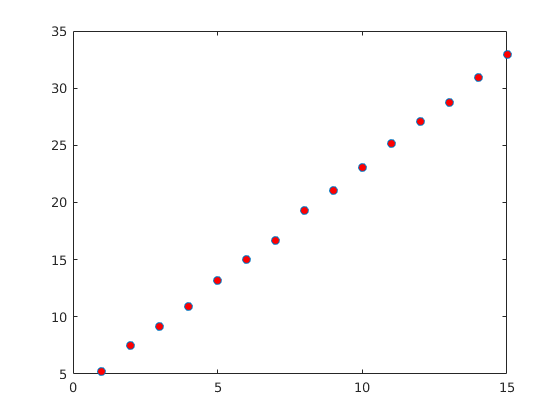
\includegraphics[width=.9\linewidth]{EjemploValidacion/dataPoints.png} 
  \end{center}}
    \only<3->{  \begin{center}
    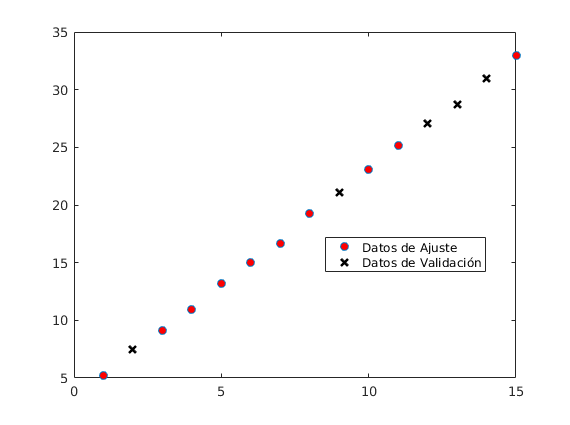
\includegraphics[width=.9\linewidth]{EjemploValidacion/dataPoints_split.png} 
  \end{center}}
  \end{minipage}
  \begin{minipage}{.28\linewidth}
	\visible<2->{Primero debemos separar nuestro set de datos}  
  \end{minipage}
  
\end{frame}


\begin{frame}{Validación: un Ejemplo}

  Realizamos el ajuste con polinomios hasta de grado $4$ para ello, podemos generalizar el  problema como: $ A \underbrace{c}_{\text{coeficientes}} = b $
donde podemos escribir

\begin{minipage}{.7\linewidth}
$$  \left[\begin{array}{*5{c}}
    \only<1-4>{n} 			& \only<1-4>{\sum x_i}  	& \only<1-3>{\sum x_i^2}	& \only<1-2>{\sum x_i^3}	& \only<1>{\sum x_i^4}\\
	\only<1-4>{\sum x_i}		& \only<1-4>{\sum x_i^2}	& \only<1-3>{\sum x_i^3}	& \only<1-2>{\sum x_i^4}	& \only<1>{\sum x_i^5}\\
	\only<1-3>{\sum x_i^2} 	& \only<1-3>{\sum x_i^3}	& \only<1-3>{\sum x_i^4}	& \only<1-2>{\sum x_i^5}	& \only<1>{\sum x_i^6}\\
    \only<1-2>{\sum x_i^3} 	& \only<1-2>{\sum x_i^4}	& \only<1-2>{\sum x_i^5}	& \only<1-2>{\sum x_i^6}	& \only<1>{\sum x_i^7}\\
	\only<1>{\sum x_i^4}		& \only<1>{\sum x_i^5} 	& \only<1>{\sum x_i^6} 	& \only<1>{\sum x_i^7} 	& \only<1>{\sum x_i^8}
	\end{array}\right]  \begin{bmatrix}
	\only<1-4>{c_0}\\
	\only<1-4>{c_1}\\
	\only<1-3>{c_2}\\
	\only<1-2>{c_3}\\
	\only<1>{c_4}
\end{bmatrix} = \begin{bmatrix}
\only<1-4>{\sum y_i}\\
\only<1-4>{\sum y_i x_i}\\
\only<1-3>{\sum y_i x_i^2}\\
\only<1-2>{\sum y_i x_i^3}\\
\only<1>{\sum y_i x_i^4}
\end{bmatrix}	  $$
\end{minipage}
\end{frame}

\begin{frame}{Validación: un Ejemplo}
Una vez hallados los coeficientes para cada caso, es posible dibujar los distintos ajustes:

\begin{minipage}{.7\linewidth}
\centering
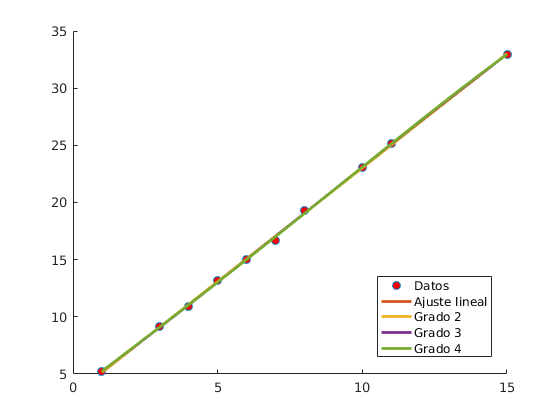
\includegraphics[width=\linewidth]{EjemploValidacion/Ajustes.png}

\end{minipage}
\begin{minipage}{.25\linewidth}
\pause Si bien parecen todos similares miremos $r^2$
\end{minipage}

\end{frame}

\begin{frame}{Validación: un Ejemplo}
  Los coeficientes de determinación
  \begin{center}
  \begin{minipage}{.6\linewidth}
    \only<1>{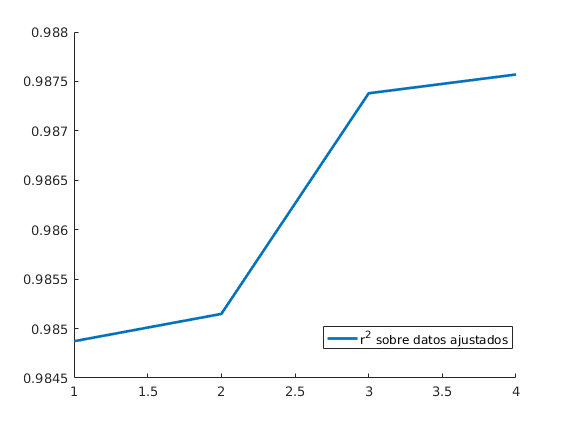
\includegraphics[width=\linewidth]{EjemploValidacion/r2_tr.png} }
    \only<2>{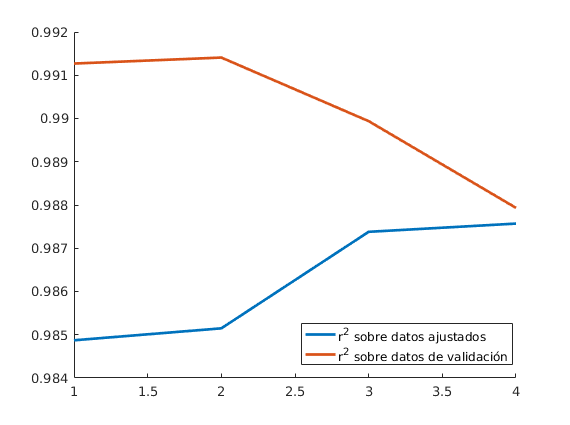
\includegraphics[width=\linewidth]{EjemploValidacion/r2_val.png} }
  \end{minipage}
  \end{center}\vspace{-3pt}  	
  \pause 
  \begin{tcolorbox}
	\textbf{Conclusión:} El mejor ajuste parece ser el cuadrático.
  \end{tcolorbox}

\end{frame}



\end{document}








